\subsection{Definitions}
Interactions between parts and robots in the assembly system are
modeled in the form of a Chemical Reaction Network (CRN).  A set of
reactions can be represented as a directed graph, ${\cal G} = ({\cal
V}, {\cal E})$. The set of vertices, ${\cal V}$, signifies the {\it
complexes}, which are the combinations of parts and/or robots that
appear before and after reaction arrows. The set of directed edges,
${\cal E}$, represents the reaction pathways between the complexes.
Each pathway is denoted by an ordered pair $(i,j) \in {\cal V}
\times {\cal V}$, which means that that complex $i$ transforms into
complex $j$, and is associated with a positive {\it reaction rate
constant}.

Each part of type $i$ in Fig. \ref{fig:assembly_plans} is symbolized
by $X_i$, and a robot is symbolized by $X_R$.  $X_i$ may be further
classified as $X_i^u$, an unclaimed part on the ground, or as
$X_i^c$, a claimed part $i$ and the robot that is carrying it. Let
$M$ be the number of these variables, or {\it species}, in a model
of the system. Then $\mathbf{x}(t) \in \mathbb{R}^M$ is the vector
of the species populations, which are represented as continuous
functions of time $t$.

\subsection{Complete macro-continuous model} % (fold)
\label{sub:complete_macro_continuous_model}

We define a CRN that represents each possible action in the
micro-continuous model of the assembly system:
\begin{eqnarray}
X_R + X_1^u ~~\xrightarrow{e_1} ~~ X_1^c &  & X_R + X_5^u ~~\xrightarrow{e_5} ~~ X_5^c \nonumber \\
X_R + X_2^u ~~\xrightarrow{e_2} ~~ X_2^c &  & X_R + X_6^u ~~\xrightarrow{e_6} ~~ X_6^c \nonumber \\
X_R + X_3^u ~~\xrightarrow{e_3} ~~ X_3^c &  & X_R + X_7^u ~~\xrightarrow{e_7} ~~ X_7^c \nonumber \\
X_R + X_4^u ~~\xrightarrow{e_4} ~~ X_4^c &  & X_R + X_8^u ~~\xrightarrow{e_8} ~~ X_8^c \nonumber \\
X_1^c + X_2^c \xrightarrow{k_1^+} X_5^c + X_R &  &  X_2^c + X_7^c \xrightarrow{k_4^+} X_{F1}^c + X_R \nonumber \\
X_3^c + X_4^c \xrightarrow{k_2^+} X_6^c + X_R & & X_2^c + X_5^c \xrightarrow{k_5^+} X_{8}^c + X_R \nonumber \\
X_5^c + X_6^c \xrightarrow{k_3^+} X_7^c + X_R & & X_6^c + X_8^c \xrightarrow{k_6^+} X_{F2}^c + X_R \nonumber \\
X_5^c \xrightarrow{k_1^-} X_1^c + X_2^u &  &  X_{F1}^c \xrightarrow{k_4^-} X_{7}^c + X_2^u \nonumber \\
X_6^c \xrightarrow{k_2^-} X_3^c + X_4^u & & X_8^c \xrightarrow{k_5^-} X_{5}^c + X_2^u\nonumber \\
X_7^c \xrightarrow{k_3^-} X_6^c + X_5^u & & X_{F2}^c
\xrightarrow{k_6^-} X_{8}^c + X_6^u
\label{eq:complete_macro_continous}
\end{eqnarray}

In this CRN, $e_i$ is the rate at which a robot encounters a part of
type $i$, $k_i^+$ is the rate of assembly process $j$, and $k_i^-$
is the rate of disassembly process $j$.  We theoretically estimate
these rates as functions of the following probabilities:
\begin{equation}
e_i = p^e~, ~~~~k_i^+ = p^e \cdot p^a_i \cdot p_i^+~, ~~~~k_i^- =
p_i^-~. \label{eq:rateDef}
\end{equation}

$p^e$ is the probability that a robot encounters a part or another
robot.  Using the assumption that robots and parts are distributed
uniformly throughout the arena, we calculate $p^e$ from the
geometrical approach that is used to compute probabilities of
molecular collisions~\cite{Gillespie:1992p8126, Correll:2006p8328}:
$p^e~\approx~v T w / A$, where $v$ is the average robot speed, $T$
is a timestep, $A$ is the area of the arena, and $w$ is twice a
robot's communication radius, since this is the range within which a
robot detects a part or robot and initiates an assembly process.

%~\cite{Gillespie:1992p8126, Puchalka:2004p4312, Turner:2004p4446,
%Correll:2007p8184, Correll:2007p8236, Correll:2006p8328}:

%the width of a robot's detection range, which is

$p^a_i$ is the probability of two robots successfully completing
assembly process $i$; it depends on the part geometries.

$p_i^+$ is the probability of two robots starting assembly process
$i$, and $p_i^-$ is the probability per unit time of a robot
performing disassembly process $i$.  These are the {\it tunable
parameters} of the system.

We compute $p^a_i$ and the parameters for $p^e$ using measurements
from the micro-continuous model (Webots simulations): $A = 23.4~
m^2$ (hexagon of radius $3~m$), $w = 1.2~ m$, $v_R = 0.128~m/s$ from
an average over $50$ runs, and $\mathbf{p^a} =
[0.9777~0.9074~0.9636~0.9737~0.8330~1.0]$ (entries follow the
numbering of the associated reactions) from averages over $100$
runs.  We set $T=1 ~s$.

In the thermodynamic limit, which includes the condition that
populations approach infinity, the physical system represented by
\eqref{eq:complete_macro_continous} can be abstracted to an ODE
model \cite{Gillespie:2007p1788}.  This is illustrated in the next
section.  We numerically integrate this macro-continuous model with
the rates we calculated and also use the StochKit
toolbox~\cite{Li:2008p11431} to efficiently perform a stochastic
simulation of the macro-discrete model.  We compare the results to
those for the micro-continuous model in Fig.
\ref{fig:img_complete_model_results}, using $p_i^+=1, ~p_i^-=0 ~~
\forall i$. The results for all models are very similar, although
discrepancies arise from two factors. First, certain events that
happen in the physical simulation are not modeled: parts sticking
together or being wedged against a wall, and deviations from the
assumption of uniform spatial distribution. Second, the ODE
approximation is valid only for large numbers of parts, and the
system modeled had only $15$ robots and $15$ parts. Overall, the
macro-continuous model accurately predicts the evolution of part
populations, and hence we can use it to design the rates to direct
the system's behavior, provided that the system has very large
numbers of parts.

%We can most effectively use it to design the rates to direct the
%system's behavior when the system contains very large numbers of
%parts.

%so our $15$-robot, $15$-part system should be expanded to most
%effectively use the ODE model as a design tool.



%and we used only $15$ robots and $15$ parts.  To most effectively
%use the ODE model as a design tool, the system should contain many
%more parts.


%However, the macro-discrete model is still accurate for even smaller
%populations (results not shown), which validates our

%arise in the physical simulation and prevent some assemblies from
%completing; these effects are not modeled. Second,

%The ODE simulation populations are incorrectly small, as we use only
%15 robots and pieces, where as the ODE approximation is valid only
%for big copy numbers.

%shows that the rates we computed closely capture the system's
%dynamics, and

%is mathematically equivalent to

%, which is based on a Gillespie Stochastic Simulation Algorithm
%\cite{Gillespie:2007p1788},




%We use the complete macro to fit the experimental data
%quantitatively under some reaction rates.

%Toward this end, we reformulate the rates as follows:

%      For chemical process, the probability of collision depends
%          on the volume swept by one molecule, which gives the probability that another
%           molecule will collide it in the next $dt$.

% $p_i^a$ can be easily measured, or assumed to be $1$ if the robots manage
% to align the pieces correctly before each assembly step.


\begin{figure}[t]
\centering
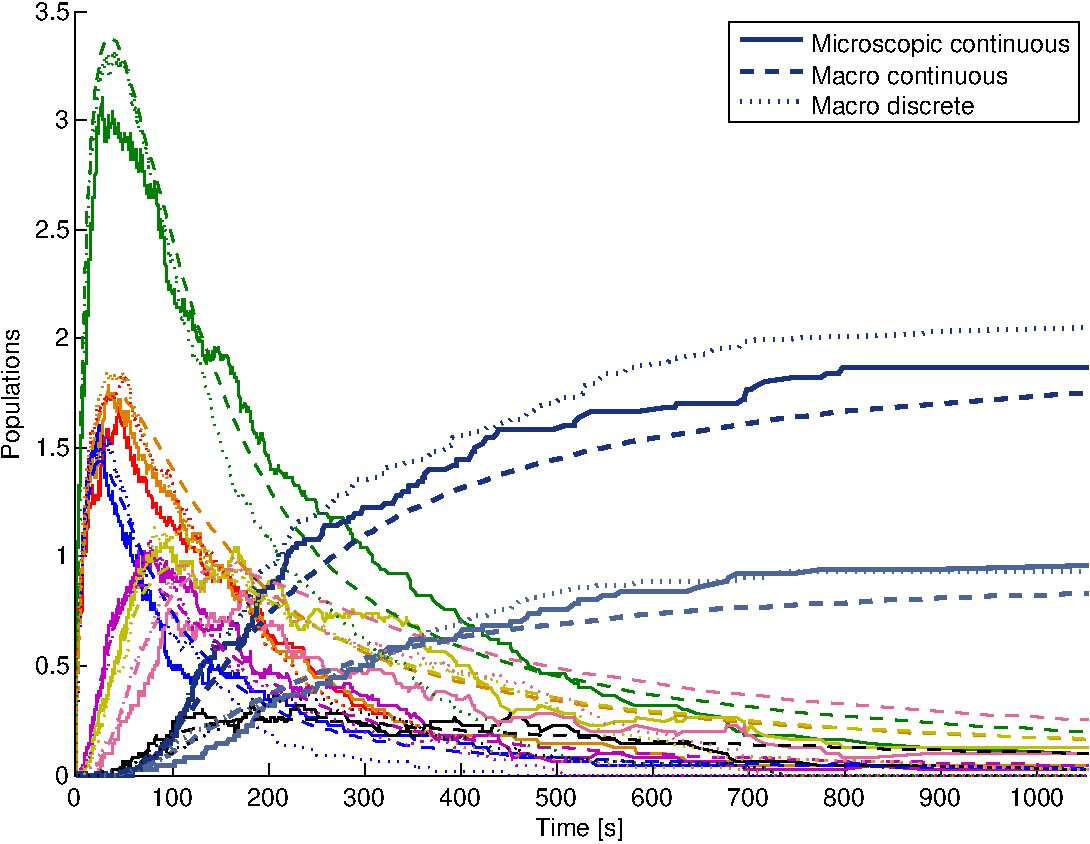
\includegraphics[width=8cm]{img/complete_model_results.pdf}
\caption{Part populations in the complete macro-continuous,
macro-discrete, and micro-continuous models for $3$ final assemblies
and $15$ robots.  Macro-discrete and micro-continuous results are
averaged over 100 runs.} \label{fig:img_complete_model_results}
\end{figure}

\subsection{Reduced macro-continuous model} % (fold)
\label{sub:simple_macro_continuous_model}
    We simplify the complete model by abstracting away robots and retaining
    only interactions between parts, assuming that the time to find a
part is small and there are more robots than parts:
    \begin{eqnarray}
        X_1 + X_2 ~~{\mathop{\rightleftharpoons}_{k_1^-}^{k_1^+}}~~ X_5 & \quad &  X_2 + X_7 ~~{\mathop{\rightleftharpoons}_{k_4^-}^{k_4^+}}~~ X_{F1} \nonumber \\
        X_3 + X_4 ~~{\mathop{\rightleftharpoons}_{k_2^-}^{k_2^+}}~~ X_6 & & X_2 + X_5 ~~{\mathop{\rightleftharpoons}_{k_5^-}^{k_5^+}}~~ X_8 \nonumber \\
        X_5 + X_6 ~~{\mathop{\rightleftharpoons}_{k_3^-}^{k_3^+}}~~ X_7 & & X_6 + X_8 ~~{\mathop{\rightleftharpoons}_{k_6^-}^{k_6^+}}~~ X_{F2}
        \label{eq:reduced_macro_continuous}
    \end{eqnarray}
    The rates are also defined by
    equation~\eqref{eq:rateDef}.

%This model should
%    converge to the same equilibria as the complete
%    model, but its transient regime differs since we removed the
%    delays that arise from robot interactions
%    with free components and other robots.

We define a vector $\mathbf{y(x)} \in \mathbb{R}^{12}$ in which
entry $y_i$ is the part or product of parts in complex $i$:
\begin{eqnarray} \mathbf{y(x)} = && [x_1
x_2~~x_5 ~~x_3 x_4 ~~x_6 ~~x_2 x_7 ~~x_{F1} \nonumber \\  && x_5
x_6~~ x_7~~x_2 x_5 ~~x_8~~ x_6 x_8 ~~x_{F2}]^T~. \label{eq:ydef1}
\end{eqnarray}
We also define a matrix $\mathbf{M} \in \mathbb{R}^{10 \times 12}$
in which each entry $M_{ji}$, $j=1,...,10$, of column $\mathbf{m}_i$
is the coefficient of part type $j$ in complex $i$ ($0$ if absent).
We relabel the rate associated with reaction $(i,j) \in \cal{E}$ as
$k_{ij}$ and define a matrix $\mathbf{K} \in \mathbb{R}^{12 \times
12}$ with entries
\begin{equation}
K_{ij} =  \left\{
\begin{array}{lll}
k_{ji} &\mbox{ if }& i \neq j~, ~~(j,i) \in \mathcal{E}~, \\
0 &\mbox{ if }& i \neq j~, ~~(j,i) \notin \mathcal{E}~,\\
-\sum_{(i,l)\in {\mathcal E}} k_{il} &\mbox{ if }& i=j~.
\end{array} \right. \label{eq:Kdef}
\end{equation}
Then our ODE abstraction of the system can be written in the
following form \cite{Chaves:2004p11839}:
\begin{equation}
\mathbf{\dot{x}} = \mathbf{M}\mathbf{K}\mathbf{y}(\mathbf{x})~.
\label{eq:matrixODE}
\end{equation}

%$K_{ij} = k_{ji}$ if $i \neq j~, (j,i) \in \mathcal{E}$; $0$ if $i
%\neq j~, (j,i) \notin \mathcal{E}$; and $-\sum_{(i,l)\in {\mathcal
%E}} k_{il}$ if $i=j$.

One set of linearly independent conservation constraints on the part
quantities is:
\begin{equation}
%\left\lbrace
\begin{array}{lll}
x_3 - x_4 &=& N_1 \\
x_1+x_5+x_7+x_8+x_{F1}+x_{F2} &=& N_2 \\
x_2+x_5+x_7+2(x_8+x_{F1}+x_{F2}) &=& N_3 \\
x_3+x_6+x_7+x_{F1}+x_{F2} &=& N_4
\end{array}
%\right.
\label{eq:cons}
\end{equation}
where $N_i$, $i=1,...,4$, are computed from the initial part
quantities.

%This simplification allows us to study the stability of this system:

\begin{theorem}\label{thm:unique_equilibrium}
System \eqref{eq:matrixODE} subject to \eqref{eq:cons} has a unique,
stable equilibrium $\mathbf{\bar{x}} > \mathbf{0}$.
\end{theorem}
\begin{proof}  Each equilibrium of the system, $\{\mathbf{\bar{x}}
~|~\mathbf{M}\mathbf{K}\mathbf{y(\bar{x})} = \mathbf{0}\}$, can be
classified as either a {\it positive} equilibrium $\mathbf{\bar{x}}
> \mathbf{0}$ or a {\it boundary} equilibrium in which $\bar{x}_i
= 0$ for some $i$, which can be found by solving
$\mathbf{y(\mathbf{\bar{x}})} =
\mathbf{0}$~\cite{Chaves:2004p11839}.  From definition
\eqref{eq:ydef1} of $\mathbf{y(x)}$, it can be concluded that in
each boundary equilibrium, all $x_i = 0$ except for one of the four
combinations of variables $(x_1,x_3), (x_1,x_4), (x_2,x_3),
(x_2,x_4)$.  Since we only consider systems that can produce
$x_{F1}$ and $x_{F2}$, it is not possible for the system to reach
any of these equilibria; each one lacks two part types needed for
the final assemblies.

%whose rows are each obtained by subtracting a column of $\mathbf{M}$
%associated with a reactant in a particular reaction from a column
%associated with a product

The {\it deficiency} $\delta$ of a reaction network is the number of
complexes minus the number of linkage classes, each of which is a
set of complexes connected by reactions, minus the network rank,
which is the rank of the matrix with rows $\mathbf{m}_i -
\mathbf{m}_j$, $(i,j) \in \cal{E}$ \cite{Feinberg:1995p9419}.
 Network \eqref{eq:reduced_macro_continuous} has $12$ complexes, $6$
linkage classes, and rank $6$; hence, $\delta = 0$.  Also, the
network is {\it weakly reversible} because whenever there is a
directed arrow pathway from complex $i$ to complex $j$, there is one
from $j$ to $i$.  Because the network has deficiency $0$, is weakly
reversible, and does not admit any boundary equilibria, it has a
unique, globally asymptotically stable positive equilibrium
according to Theorem 4.1 of \cite{Siegel:2000}.
\end{proof}

%These properties, along with the fact that the system kinetics are
%mass-action, satisfy the criteria for applying the Deficiency Zero
%Theorem \cite{Feinberg:1995p9419}, which gives the result that the
%system has exactly one positive steady state, which is
%asymptotically stable.  In fact, by Theorem 4.1 of
%\cite{Siegel:2000}

%\cite{Feinberg:1987p9428}

% subsection simple_macro_continuous_model (end)